\chapter{Prodotto finale}
\label{cap:prodotto-finale}

\intro{Il seguente capitolo ha la funzione di illustrare il prodotto realizzato in tutte le sue componenti.}

\setlength{\parskip}{3ex}

\section{Menu}
\begin{figure}[!h]
\centering
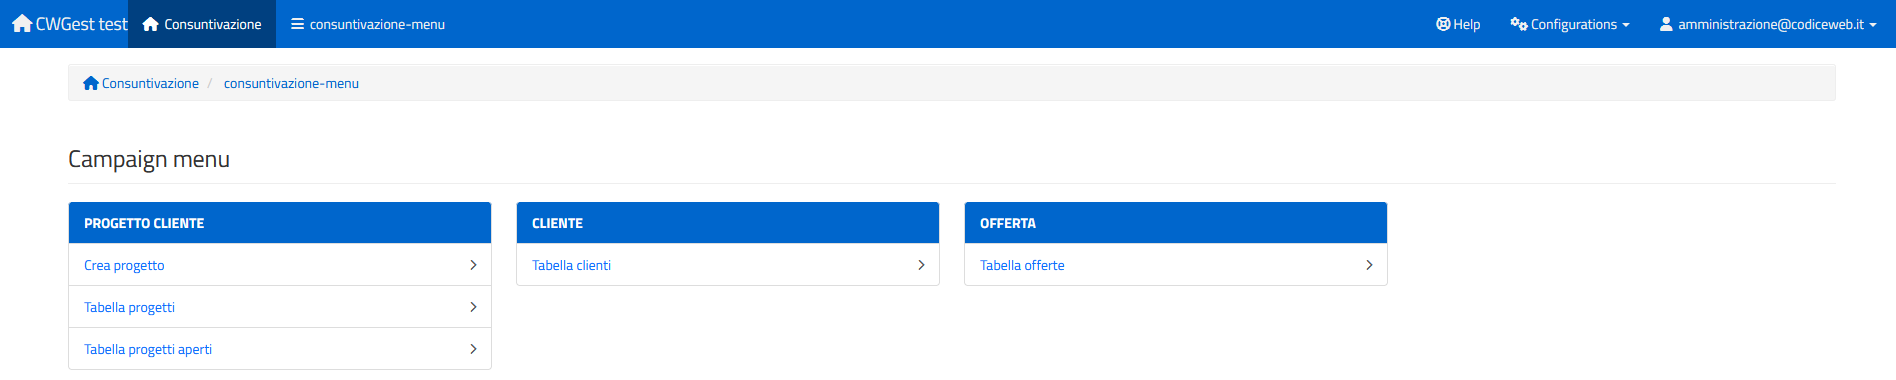
\includegraphics[width=380px]{../images/UI/01-menu.png}
\caption{Modulo Campaign: Menu}
\label{fig:menu}
\end{figure}

\noindent Il menu ({\hyperref[fig:menu]{figura 6.1}}) mette a disposizione dell'utente tutte le funzionalità del modulo \textbf{Campaign}. Tra le operazioni che l'utente può svolgere troviamo:
\begin{itemize}
\item creazione di un nuovo progetto;
\item accesso alla tabella dei progetti;
\item accesso alla tabella dei progetti aperti;
\item accesso alla tabella dei clienti;
\item accesso alla tabella delle offerte.
\end{itemize}

\pagebreak

\section{Creazione di un progetto}
\begin{figure}[!h]
\centering
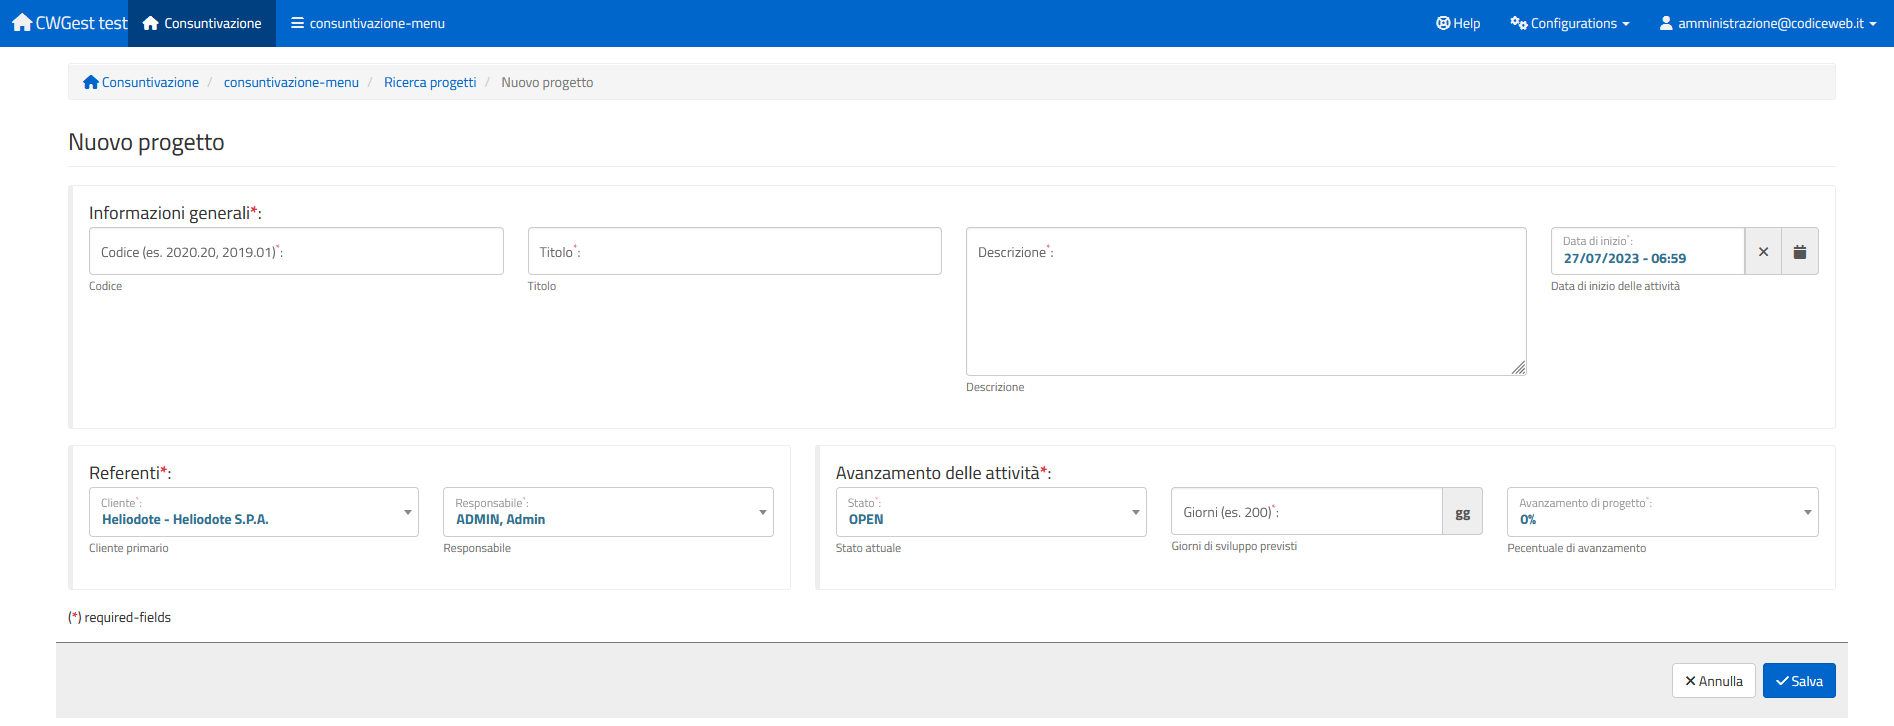
\includegraphics[width=380px]{../images/UI/02-nuovoProgetto.png}
\caption{Modulo Campaign: Creazione di un progetto}
\label{fig:nuovoProgetto}
\end{figure}

\noindent La pagina di creazione di un progetto ({\hyperref[fig:nuovoProgetto]{figura 6.2}}), raggiungibile dal menu ({\hyperref[fig:menu]{figura 6.1}}) o dalla tabella dei progetti ({\hyperref[fig:tabellaProgetti]{figura 6.3}}), mette a disposizione dell'utente un form composto da una serie di campi, tutti obbligatori, che devono essere compilati per creare il progetto. Tali campi sono i seguenti:
\begin{itemize}
\item codice identificativo;
\item titolo;
\item descrizione;
\item data di inizio dell'attività di sviluppo;
\item cliente proponente (CWBI o altro);
\item responsabile assegnato al progetto;
\item stato attuale (aperto, chiuso, approvato, rifiutato, sospeso);
\item giorni di sviluppo previsti per portare a termine il progetto;
\item percentuale di avanzamento del progetto.
\end{itemize}

\pagebreak

\section{Tabella progetti}
\begin{figure}[!h]
\centering
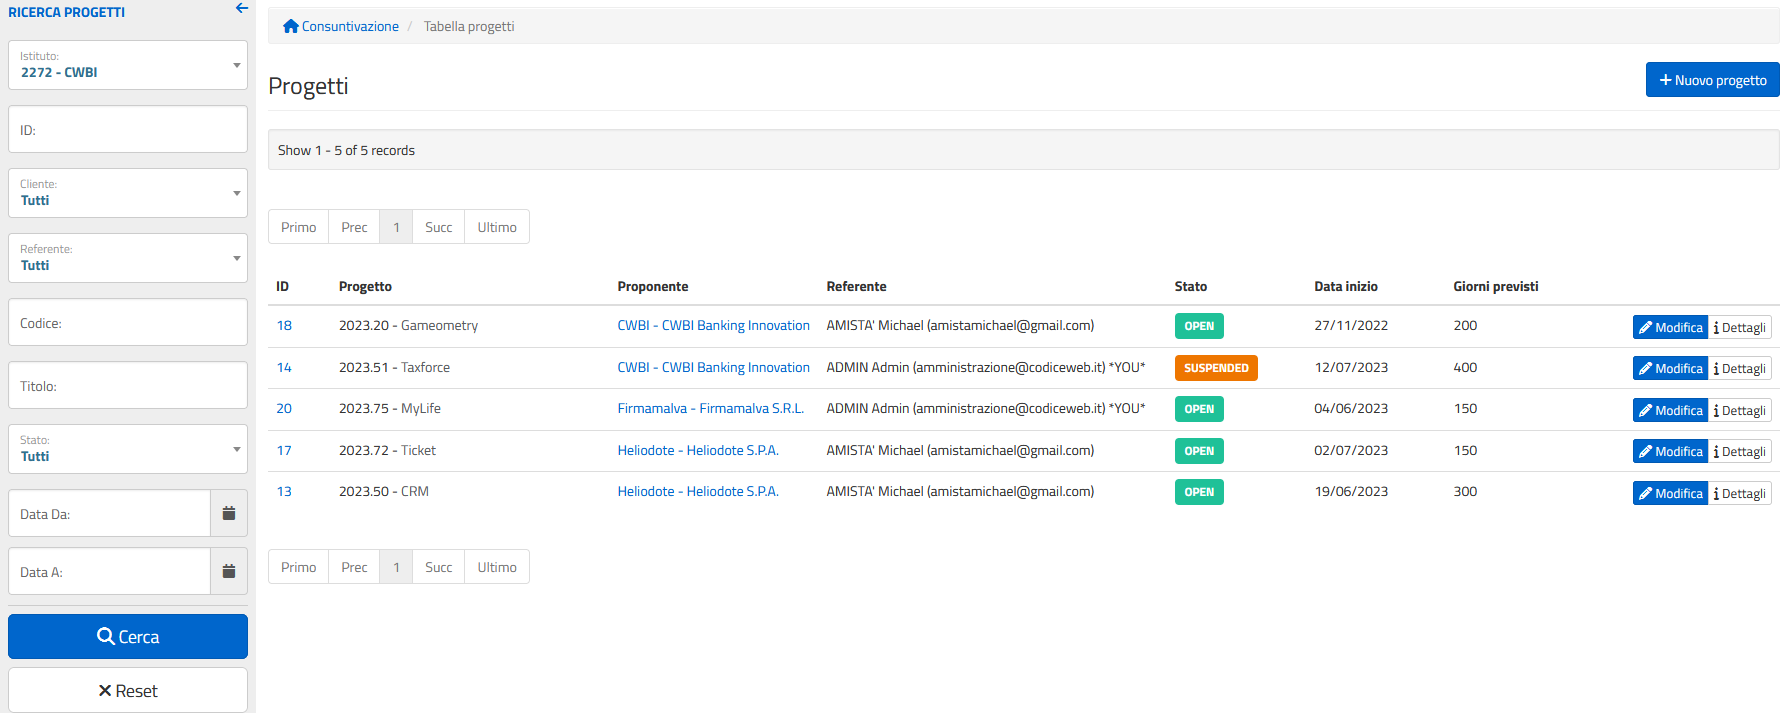
\includegraphics[width=380px]{../images/UI/03-tabellaProgetti.png}
\caption{Modulo Campaign: Tabella progetti}
\label{fig:tabellaProgetti}
\end{figure}

\noindent La tabella dei progetti ({\hyperref[fig:tabellaProgetti]{figura 6.3}}) consente all'utente di:
\begin{itemize}
\item visualizzare la lista completa dei progetti presenti nel sistema. Per ogni progetto visualizzato è possibile inoltre: 
\begin{itemize}
\item modificare il progetto in linea aprendo la pagina in  {\hyperref[fig:nuovoProgetto]{figura 6.2}} con l'unica differenza che i campi saranno precompilati con i valori del progetto memorizzato;
\item visualizzare il dettaglio del progetto in linea ({\hyperref[fig:dettaglioProgetto]{figura 6.4}}).
\end{itemize}

\item creare un nuovo progetto;
\item ricercare uno o più progetti tramite il form di ricerca composto dai seguenti campi tutti opzionali:
\begin{itemize}
\item istituto, campo standard presente in tutti i form di ricerca dell'azienda. Consente di ricerca progetti correlati ad una delle sedi di CWBI;
\item ID del progetto, assegnato dal database;
\item cliente;
\item codice;
\item titolo;	
\item stato attuale;
\item data di creazione.
\end{itemize}
L'utente può inoltre cancellare i dati inseriti nel form di ricerca tramite l'opzione \textit{Reset} e effettuare la ricerca tramite l'opzione \textit{Cerca}.
\end{itemize}

\pagebreak

\section{Dettaglio di un progetto}
\begin{figure}[!h]
\centering
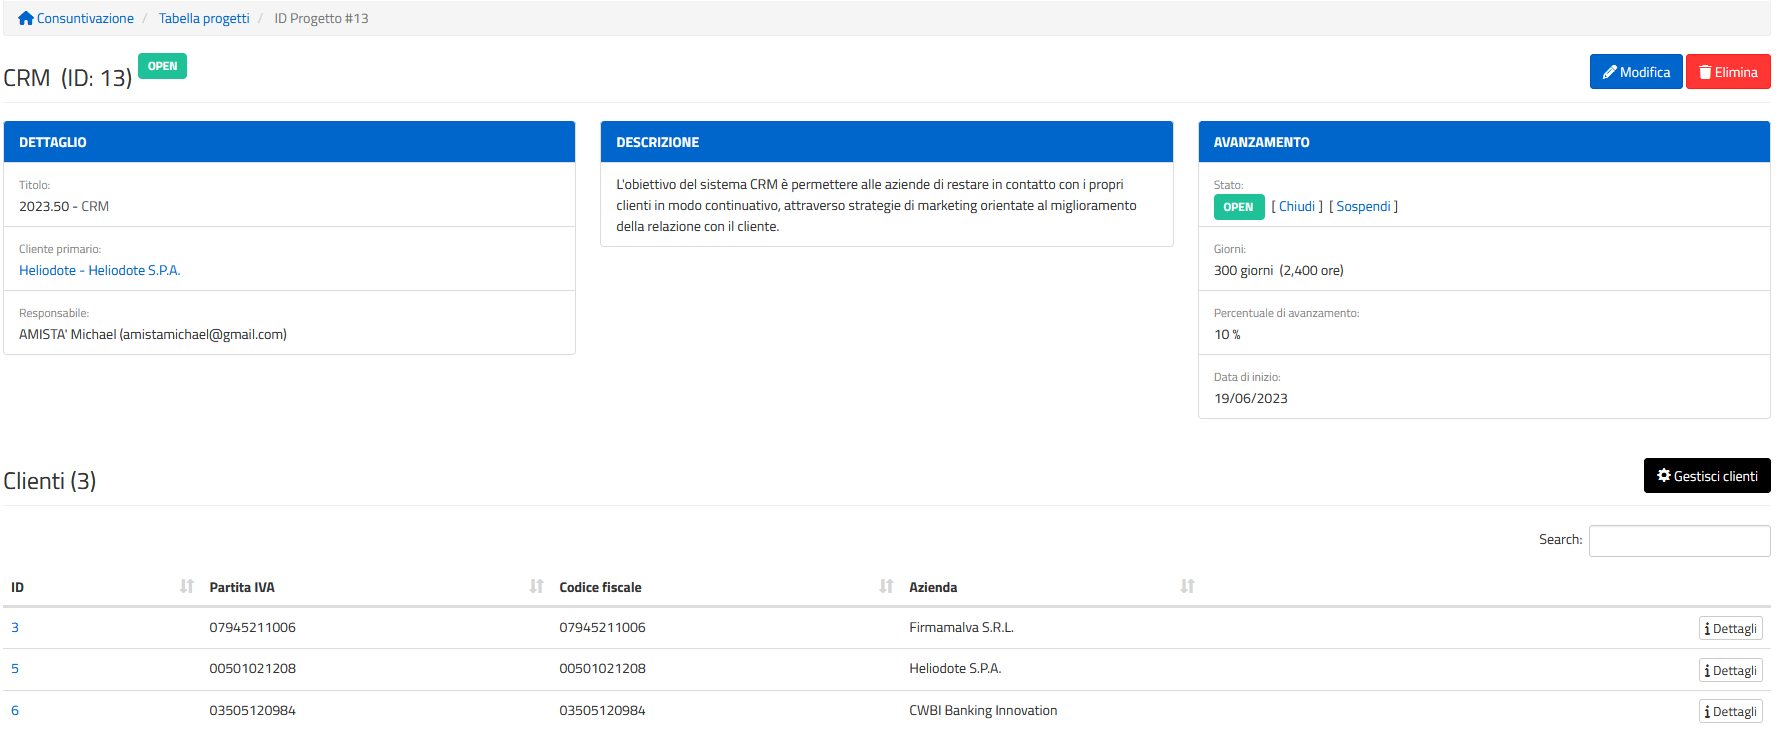
\includegraphics[width=380px]{../images/UI/04-dettaglioProgetto.png}
\caption{Modulo Campaign: Dettaglio di un progetto}
\label{fig:dettaglioProgetto}
\end{figure}

\noindent La pagina di dettaglio di un progetto ({\hyperref[fig:dettaglioProgetto]{figura 6.4}}) consente all'utente di visualizzare i dettagli di un progetto selezionato. Nella pagina sono presenti i medesimi dati inseriti in fase di creazione del progetto. Nella pagina sono presenti le funzionalità di \textit{modifica} ed \textit{eliminazione} del progetto. È inoltre presente una tabella che mostra l'elenco di tutti i clienti interessati al progetto. 

\begin{figure}[!h]
\centering
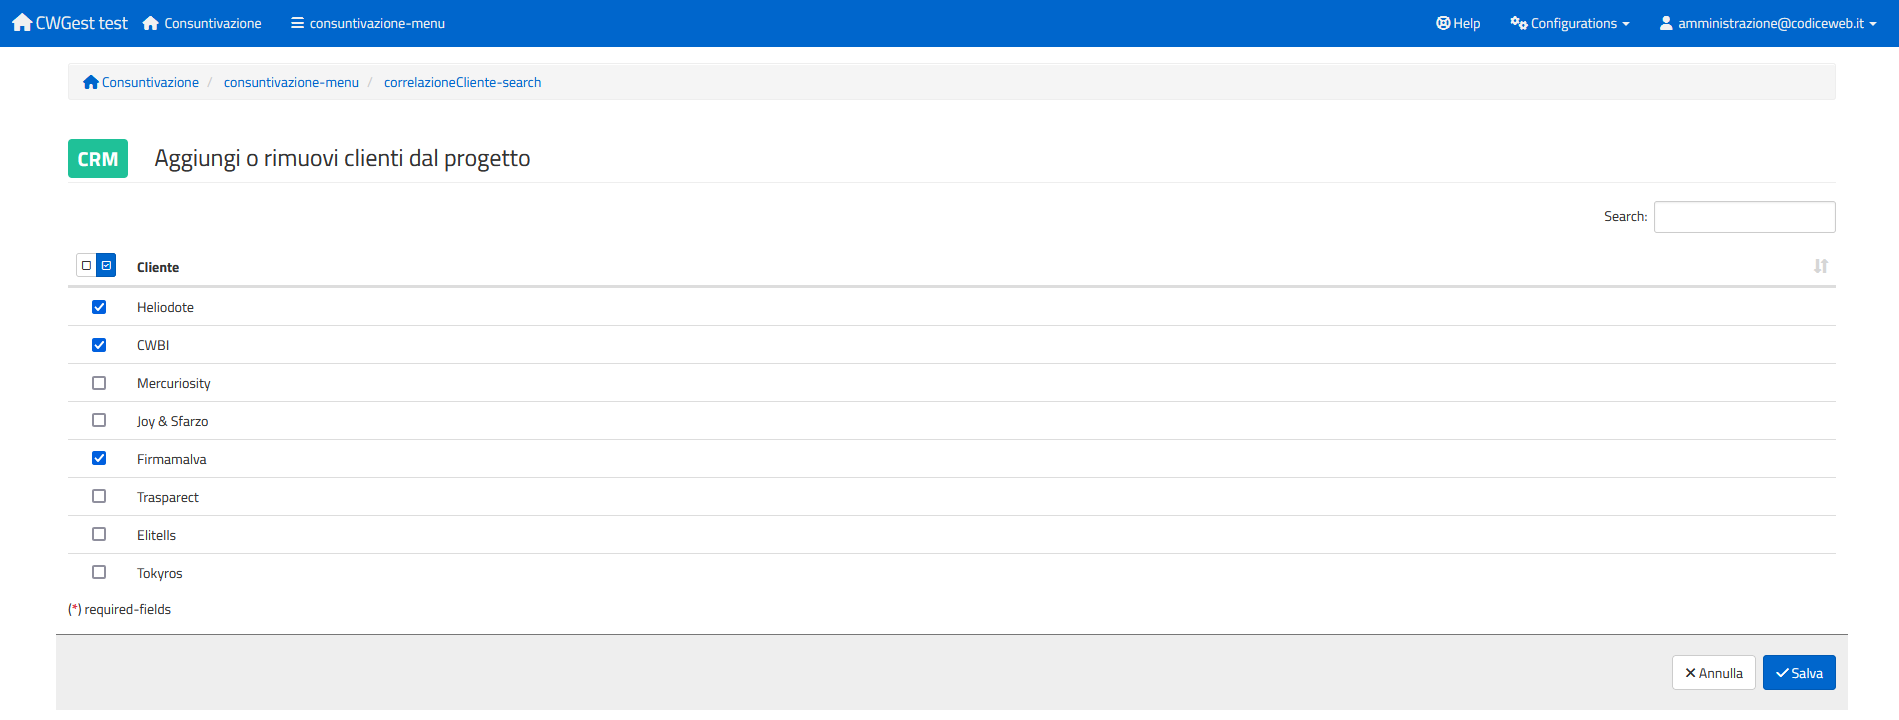
\includegraphics[width=380px]{../images/UI/06-aggiungiRimuoviClienti.png}
\caption{Modulo Campaign: Dettaglio di un progetto - Gestione clienti}
\label{fig:gestioneClienti}
\end{figure}

\noindent Tramite la funzionalità \textit{Gestione clienti} presente nella pagina di dettaglio di un progetto ({\hyperref[fig:gestioneClienti]{figura 6.5}}) si arriva alla pagina ({\hyperref[fig:dettaglioProgetto]{figura 6.4}}) che consente di aggiungere e rimuovere i clienti interessati al progetto.

\pagebreak

\section{Tabella progetti aperti}
\begin{figure}[!h]
\centering
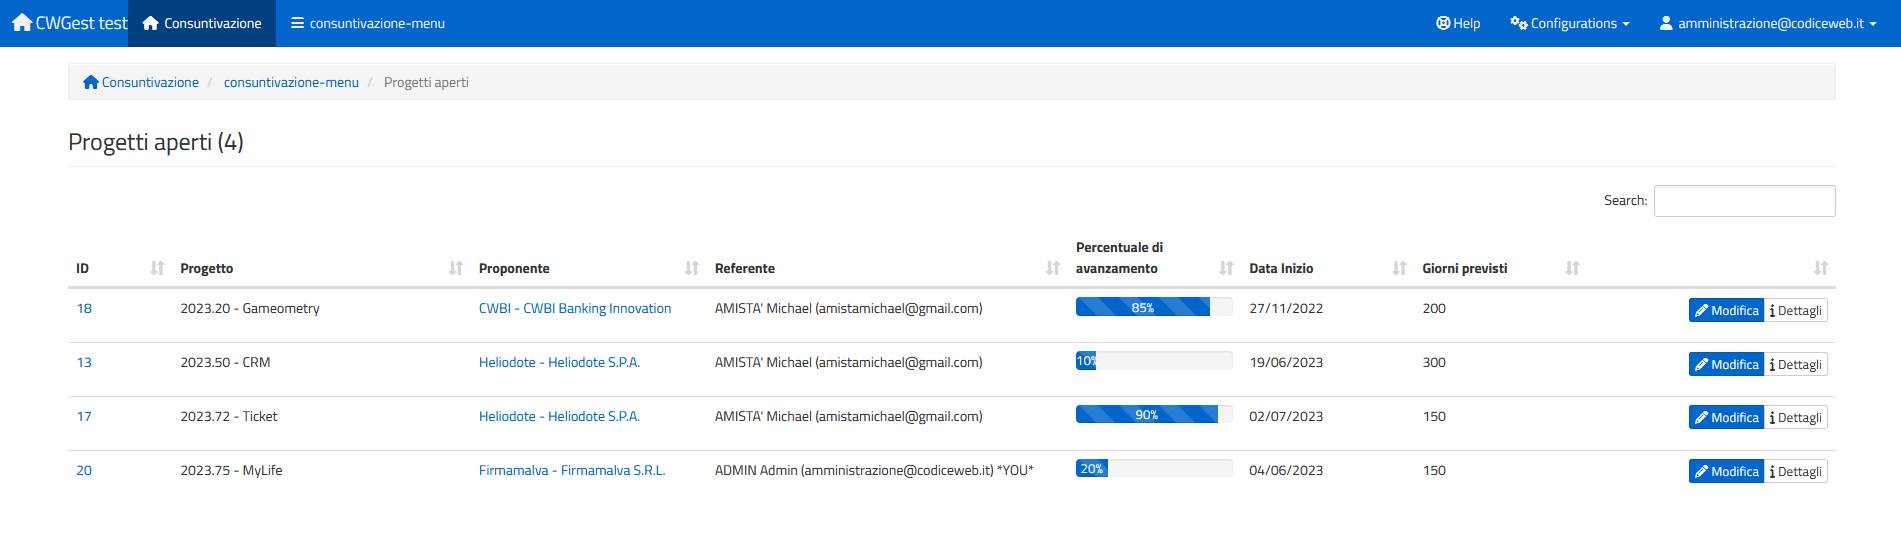
\includegraphics[width=380px]{../images/UI/07-tabellaProgettiAperti.png}
\caption{Modulo Campaign: Tabella progetti aperti}
\label{fig:tabellaProgettiAperti}
\end{figure}

\noindent La tabella dei progetti aperti ({\hyperref[fig:tabellaProgettiAperti]{figura 6.6}}) consente all'utente di visualizzare la lista di tutti i progetti ancora aperti. Oltre che visualizzare i dati principali dei progetti in elenco, consente per ciascun progetto in linea di accedere alla pagina di modifica e alla pagina di dettaglio ({\hyperref[fig:dettaglioProgetto]{figura 6.4}}).  

\pagebreak

\section{Tabella clienti}
\begin{figure}[!h]
\centering
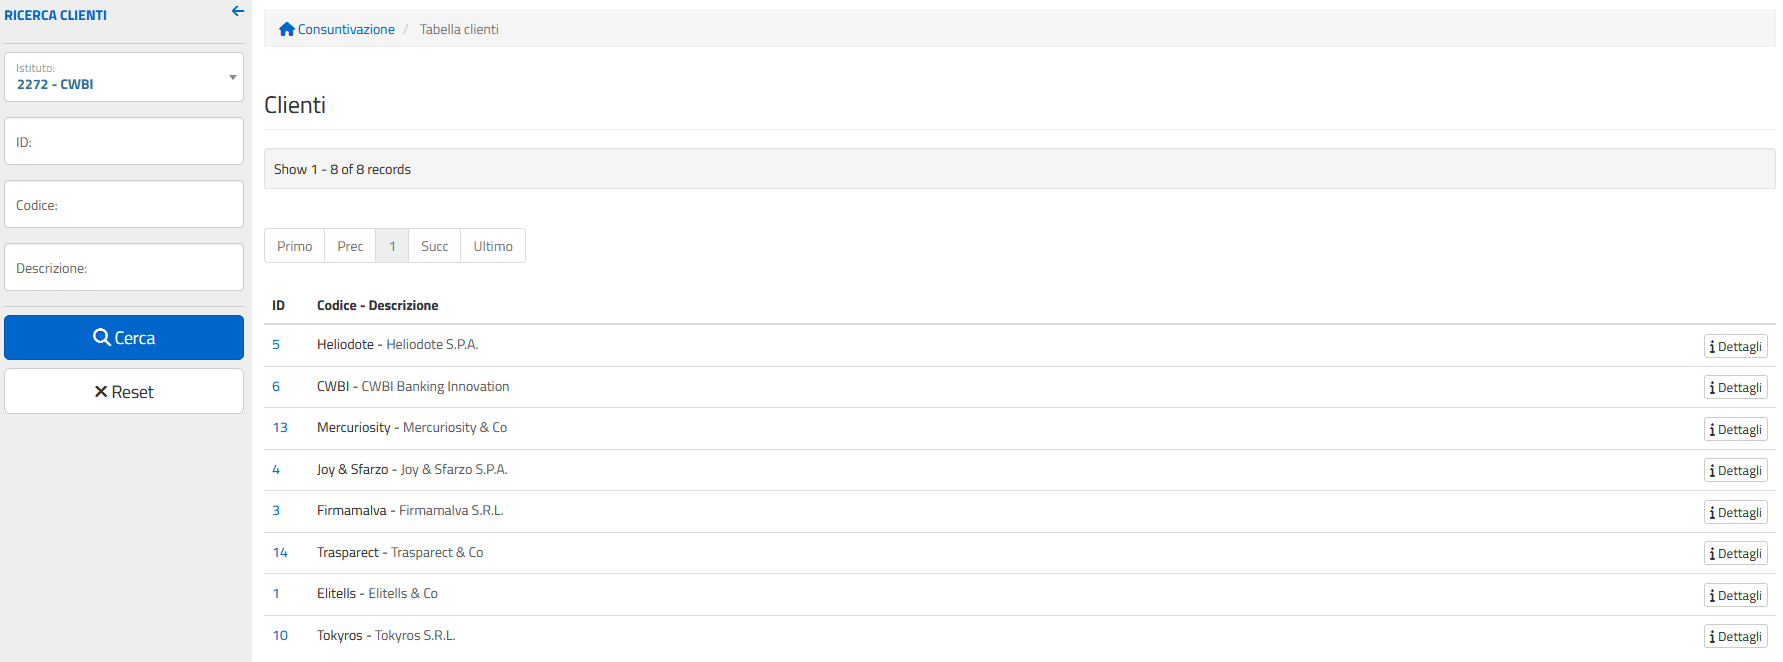
\includegraphics[width=380px]{../images/UI/08-tabellaClienti.png}
\caption{Modulo Campaign: Tabella clienti}
\label{fig:tabellaClienti}
\end{figure}

\noindent La tabella dei clienti ({\hyperref[fig:tabellaClienti]{figura 6.7}}) consente all'utente di:
\begin{itemize}
\item visualizzare la lista completa dei clienti presenti nel sistema. Per ogni cliente visualizzato è possibile accedere alla sua pagina di dettaglio (INSERIRE FIGURA); 
\item ricercare uno o più clienti tramite il form di ricerca composto dai seguenti campi tutti opzionali:
\begin{itemize}
\item istituto, campo standard presente in tutti i form di ricerca dell'azienda. Consente di ricerca progetti correlati ad una delle sedi di CWBI;
\item ID del cliente, assegnato dal database;
\item codice, nome dell'azienda;
\item descrizione, nome esteso dell'azienda.
\end{itemize}
L'utente può inoltre cancellare i dati inseriti nel form di ricerca tramite l'opzione \textit{Reset} e effettuare la ricerca tramite l'opzione \textit{Cerca}.
\end{itemize}

\pagebreak

\section{Dettaglio di un cliente}
\noindent La pagina di dettaglio di un cliente consente di visualizzare, oltre ai dati di un cliente, due schede:
\begin{enumerate}
\item progetti associati ({\hyperref[fig:dettaglioCliente1]{figura 6.8}}), corrisponde a tutti i progetti correlati al cliente e suddivisi in base allo stato del progetto stesso;
\item offerte associate ({\hyperref[fig:dettaglioCliente2]{figura 6.9}}), corrisponde a tutte le offerte formulate al cliente e relative ad uno dei progetti a cui è/era associato.
\end{enumerate}

\begin{figure}[!h]
\centering
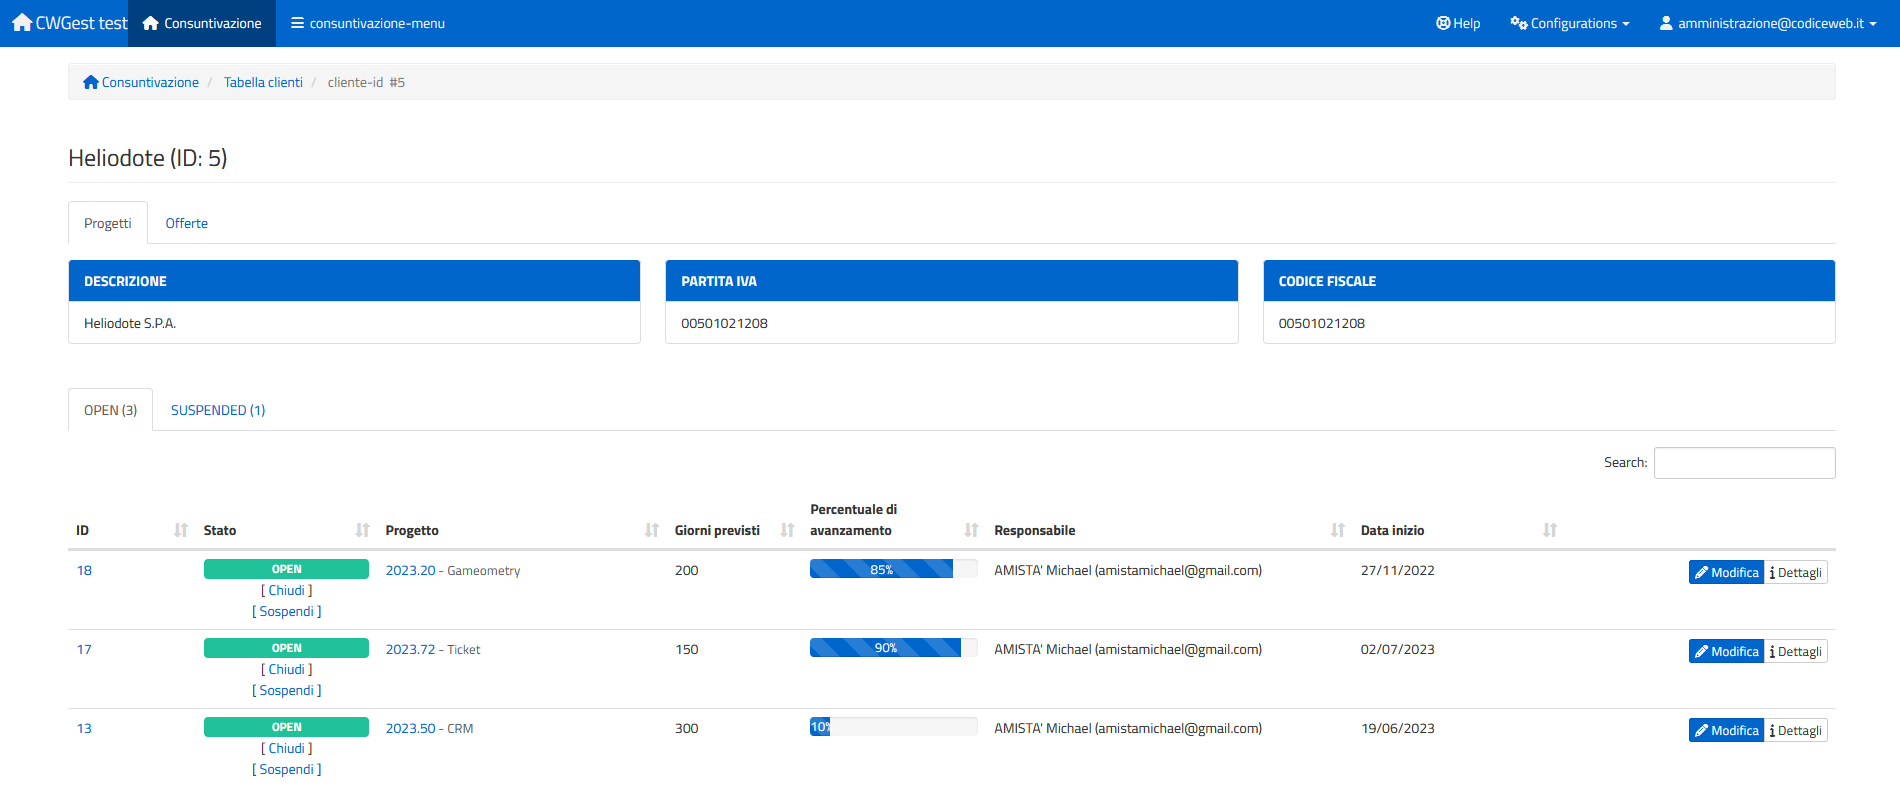
\includegraphics[width=380px]{../images/UI/09-dettaglioClienteTab1.png}
\caption{Modulo Campaign: Dettaglio di un cliente - Scheda progetti associati}
\label{fig:dettaglioCliente1}
\end{figure} 

\begin{figure}[!h]
\centering
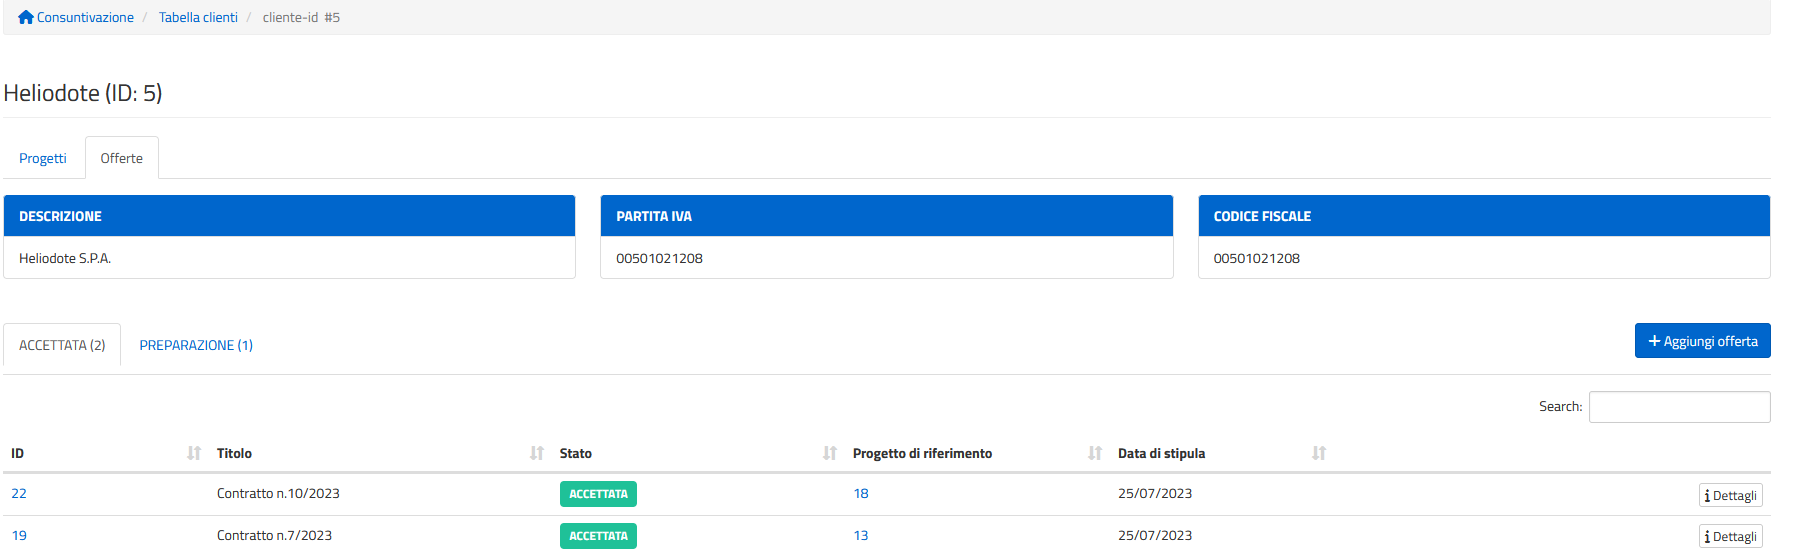
\includegraphics[width=380px]{../images/UI/09-dettaglioClienteTab2.png}
\caption{Modulo Campaign: Dettaglio di un cliente - Scheda offerte associate}
\label{fig:dettaglioCliente2}
\end{figure}

\noindent Nella scheda delle offerte ({\hyperref[fig:dettaglioCliente2]{figura 6.9}}), oltre a visualizzare tutte le offerte formulate per il cliente selezionato, è possibile creare una nuova offerta per il cliente.

\pagebreak

\begin{figure}[!h]
\centering
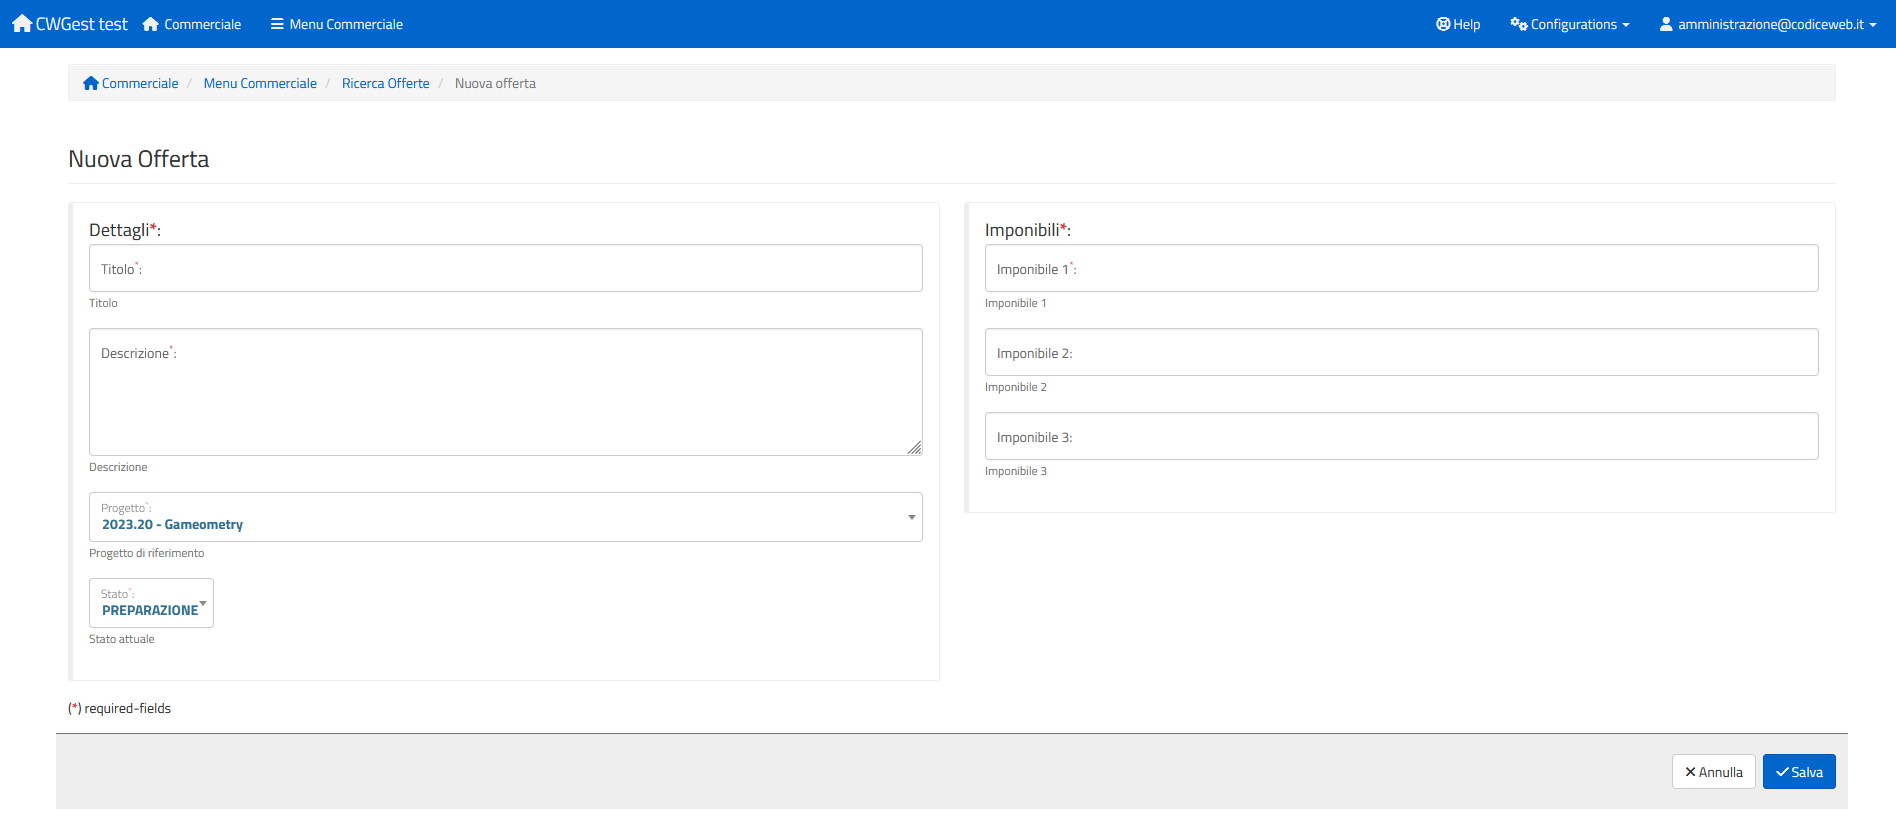
\includegraphics[width=380px]{../images/UI/10-nuovaOfferta.png}
\caption{Modulo Campaign: Dettaglio di un cliente - Aggiungi offerta}
\label{fig:nuovaOfferta}
\end{figure}

\noindent Nella pagina della nuova offerta ({\hyperref[fig:nuovaOfferta]{figura 6.10}}) l'utente ha la possibilità di aggiungere una nuova offerta per il cliente selezionato in precedenza nella pagina in {\hyperref[fig:dettaglioCliente2]{figura 6.9}}. \\
I campi che compongono la nuova offerta sono i seguenti:
\begin{itemize}
\item titolo;
\item descrizione;
\item progetto su cui formulare l'offerta. Alla lista dei progetti selezionabili corrispondono i progetti associati al cliente in questione e visibili nella scheda dei progetti associati della pagina di dettaglio del cliente ({\hyperref[fig:dettaglioCliente1]{figura 6.8}}). 
\item stato (in preparazione, in accettazione, accettata);
\item imponibile 1, corrispondente al primo prezzo formulato al cliente per il progetto selezionato;
\item imponibile 2, corrispondente al secondo prezzo formulato al cliente per il progetto selezionato;
\item imponibile 3, corrispondente al terzo prezzo formulato al cliente per il progetto selezionato.
\end{itemize}

\pagebreak

\section{Tabella offerte}

\pagebreak

\section{Dettaglio di un'offerta}
